\documentclass[10pt]{article}

\usepackage{amsthm}
\usepackage{amsmath}
\usepackage{amssymb}
\usepackage{mathtools}
\usepackage{graphicx}
\usepackage[colorinlistoftodos]{todonotes}
\usepackage{url}
\usepackage{xcolor}
\usepackage[font=small,labelfont=bf]{caption}

\usepackage{pgfplots}

\usepackage[left = 1cm, top = 1cm, bottom = 2cm, right = 1cm, nohead, nofoot]{geometry}

\pgfplotsset{width=20cm, compat=1.9}

\newcommand{\C}{\mathbb{C}}  % Complex
\newcommand{\R}{\mathbb{R}}  % Real
\newcommand{\Z}{\mathbb{Z}}  % Integers
\newcommand{\N}{\mathbb{N}}  % Naturals

\newcommand{\A}{\mathbb{A}}
\newcommand{\K}{\mathbb{K}}

\title{$\A$dvanced $\C$alculus}
\author{$\C$ason $\K$onzer}
\date{December 2, 2021}



\begin{document}
\maketitle

\newpage

%%%%%%%%%%%%%%%%%%%%%%%%%%%%%%%%%%%%%%%%%%%%%%%%%%%%%%%%%%%%%%%%%%%%%%%%%%%%%%%%%%%%%%%%%%%%%%%%
%%%%%%%%%%%%%%%%%%%%%%%%%%%%%%%%%%        Problem #1       %%%%%%%%%%%%%%%%%%%%%%%%%%%%%%%%%%%%%
\section{\underline{}}
\label{sec: Problem 1}

\noindent
Find the Fourier integral representation of the solution, $ u(x,t) $, 
to the heat equation on a metal bar of infinite length in both directions, 
with arbitrary $ c $ and $ u(x,0) = f(x) = e^{-|x|} $. Simplify the inner integral. \\
\vspace{2.5mm}

\hrule 

\vspace{7.5mm}

\begin{itemize}
    \item Solve for $ \displaystyle A(p) = \dfrac{1}{\pi} \int_{-\infty}^{\infty} f(v)\cos{pv} \,dv $.
    \subitem $ \displaystyle A(p) = \dfrac{1}{\pi} \int_{-\infty}^{\infty} e^{-|x|}\cos{pv} \,dv $
    \subitem $ \displaystyle A(p) = \dfrac{2}{\pi(p^2 + 1)} $ ; Integration in notebook. 
    \item Solve for $ \displaystyle B(p) = \dfrac{1}{\pi} \int_{-\infty}^{\infty} f(v)\sin{pv} \,dv $.
    \subitem $ \displaystyle B(p) = \dfrac{1}{\pi} \int_{-\infty}^{\infty} e^{-|x|}\sin{pv} \,dv $
    \subitem $ \displaystyle B(p) = 0 $ ; Integration in notebook.
    \item Substitute $ A(p), B(p) $ into $ \displaystyle u(x,t) = \int_{0}^{\infty} \Bigl[ A(p)\cos{px} + B(p)\sin{px} \Bigr] e^{-c^2p^2t} \, dp $.
    \subitem $ \displaystyle u(x,t) = \dfrac{2}{\pi} \int_{0}^{\infty} \Bigl[ \dfrac{\cos{px}}{(p^2 + 1)} \Bigr] e^{-c^2p^2t} \, dp $
\end{itemize}

\newpage

%%%%%%%%%%%%%%%%%%%%%%%%%%%%%%%%%%%%%%%%%%%%%%%%%%%%%%%%%%%%%%%%%%%%%%%%%%%%%%%%%%%%%%%%%%%%%%%%
%%%%%%%%%%%%%%%%%%%%%%%%%%%%%%%%%%        Problem #2       %%%%%%%%%%%%%%%%%%%%%%%%%%%%%%%%%%%%%
\section{\underline{}}
\label{sec: Problem 2}

\noindent
Use Mathematica to plot your solution from \#1 (with $ c = 1 $), 
plotting $ u(x,0) $, $ u(x,1) $, and $ u(x,2) $ on the same graph. \\
\vspace{2.5mm}

\hrule 

\vspace{7.5mm}

\begin{center}
    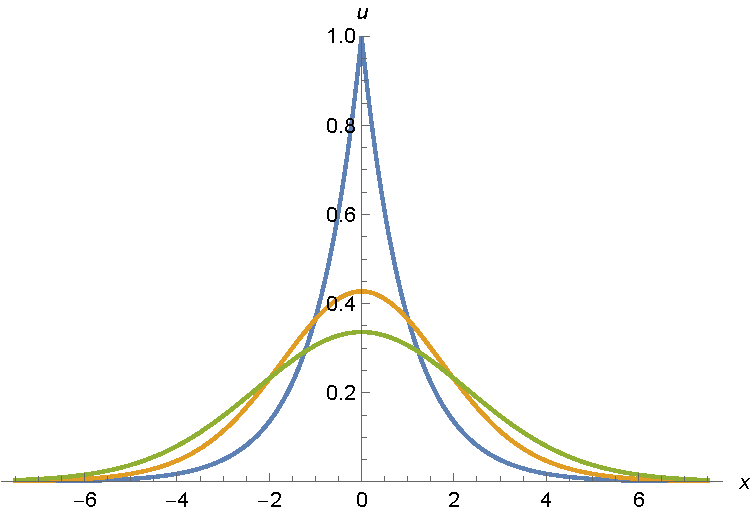
\includegraphics[width=0.8\textwidth]{img/2_1.pdf}
    \vspace{7.5mm}
    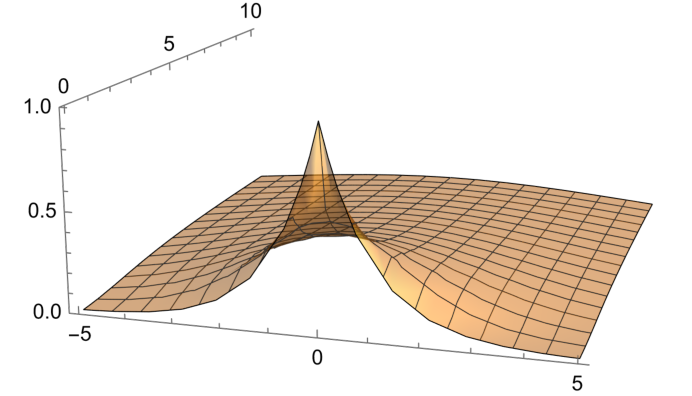
\includegraphics[width=0.8\textwidth]{img/2_2.pdf}
\end{center}

\newpage

%%%%%%%%%%%%%%%%%%%%%%%%%%%%%%%%%%%%%%%%%%%%%%%%%%%%%%%%%%%%%%%%%%%%%%%%%%%%%%%%%%%%%%%%%%%%%%%%
%%%%%%%%%%%%%%%%%%%%%%%%%%%%%%%%%%        Problem #3       %%%%%%%%%%%%%%%%%%%%%%%%%%%%%%%%%%%%%
\section{\underline{}}
\label{sec: Problem 3}

\noindent
Find the Fourier integral representation of the solution, $ u(x,t) $, 
to the heat equation on a half-infinite metal bar of, with arbitrary $ c $, 
$ u(0,t) = 0 $, and $ u(x,0) = f(x) = Boole[0 < x < 2] (1 - (x - 1)^2) $. 
Simplify the inner integral.  \\
\vspace{2.5mm}

\hrule 

\vspace{7.5mm}

\begin{itemize}
    \item Solve for $ \displaystyle \hat{f_{s}}(w) = \int_{0}^{\infty} f(p)\sin{wp} \,dp $.
    \subitem $ \displaystyle \hat{f_{s}}(w) = \int_{0}^{2} (1-(p-1)^2)\sin{wp} \,dp $
    \subitem $ \displaystyle \hat{f_{s}}(w) = -\dfrac{4\sin{(w)}(w\cos{(w)} -\sin{(w)})}{w^{3}} $ ; Integration in notebook. 
    \item Substitute $ \hat{f_{s}}(w) $ into $ \displaystyle u(x,t) = \int_{0}^{\infty} \hat{f_{s}}(w) \sin{(wx)} e^{-c^2w^2t} \, dw $.
    \subitem $  \displaystyle u(x,t) = \dfrac{2}{\pi} \int_{0}^{\infty} -\dfrac{4\sin{(w)}(w\cos{(w)} -\sin{(w)})}{w^{3}} \sin{(wx)} e^{-c^2w^2t} \, dw $
    \item Simplify the solution.
    \subitem $  \displaystyle u(x,t) = -\dfrac{8}{\pi} \int_{0}^{\infty} \dfrac{\sin{(w)}(w\cos{(w)} -\sin{(w)})}{w^{3}} \sin{(wx)} e^{-c^2w^2t} \, dw $
\end{itemize}

\newpage


%%%%%%%%%%%%%%%%%%%%%%%%%%%%%%%%%%%%%%%%%%%%%%%%%%%%%%%%%%%%%%%%%%%%%%%%%%%%%%%%%%%%%%%%%%%%%%%%
%%%%%%%%%%%%%%%%%%%%%%%%%%%%%%%%%%        Problem #4       %%%%%%%%%%%%%%%%%%%%%%%%%%%%%%%%%%%%%
\section{\underline{}}
\label{sec: Problem 4}

\noindent
Use Mathematica to plot your solution from \#3 (with $ c = 1 $), 
plotting $ u(x,0) $ and $ u(x,0.5) $ on the same graph. \\
\vspace{2.5mm}

\hrule 

\vspace{7.5mm}

\begin{center}
    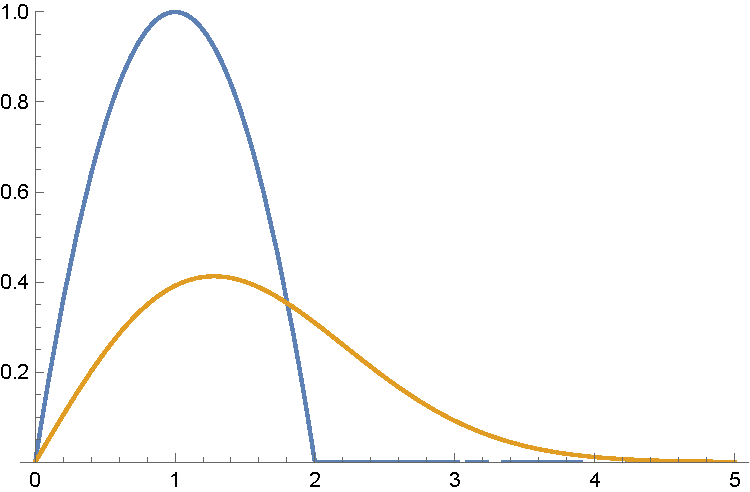
\includegraphics[width=0.8\textwidth]{img/4_1.pdf}
    \vspace{7.5mm}
    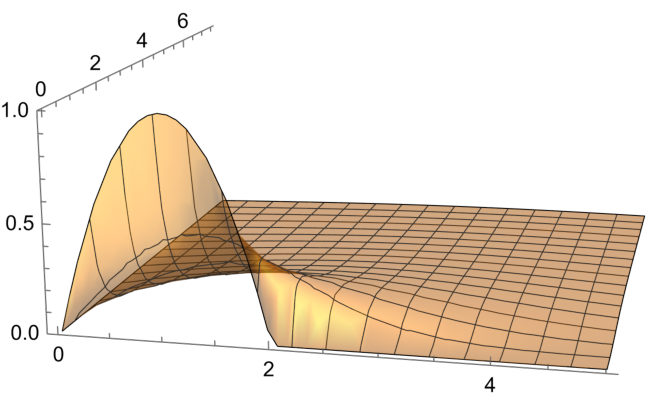
\includegraphics[width=0.8\textwidth]{img/4_2.pdf}
\end{center}

\newpage

\end{document}


%%%%%%%%%%%%%%%%%%%%%%%%%%%%%%%%%%%%%%%%%%%%%%%%%%%%%%%%%%%%%%%%%%%%%%%%%%%%%%%%%%%%%%%%%%%%%%%%
%%%%%%%%%%%%%  Comments - December 2, 2021 Advanced Calculus Written Home Work #7  %%%%%%%%%%%%%